\documentclass[main.tex]{subfiles}
\begin{document}
  \section{The Model}
    \subsection{Design and Development}
      \lipsum[4]
    \subsection{Mathematical Representation}
      \lipsum[5]
    \subsection{Implementation in Mathematica}
      \lipsum[6]
    \subsection{temporary section}
    
      \begin{SCfigure}
        \centering
        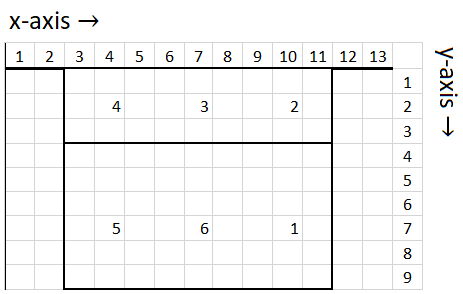
\includegraphics[width=0.5\linewidth]{figures/playingFieldGridLabelled}
        \caption{The coordinate system laid over the playing field. The net is spun at y=0 in the figure. \\
          This system is primarily used to allow the model to take player positions into account, like the distance that the setter must cover to reach the ball from their position. \\
          It is also used when noting down real world data to a format that the model can interpret.}
        \label{fig:field}
      \end{SCfigure}
      
      \begin{table}[h!]
        \label{tab:positions}
        \centering
        \caption{Basic constants defined for each position. \\
          Each position is assigned a number of constants that help calculate parameters that are in turn used to score the different positions. \\
          Note that Position 0 either refers to the setter's coordinates or to a "Dump", an attack by the setter without first setting to another player. \\
          Starting Coordinates refers to the coordinates that the setter would start from when in this position, which informs how far they have to run to reach the ball and hence how difficult the set is to perform. \\
          Ideal Contact Coordinates describe where a player or the setter would be if they contact the ball in the ideal position. While the setter may not always be in this position, it is assumed for the model that all other players are in their ideal position when the setter makes their decision. \\
          Bias Difficulty is used to tune the model. It was observed for example that positions closer to the net are more likely to be set to, as they are easier to attack from successfully.}
        \begin{tabular}{ c | c c c }
          \hline
          Position & Starting Coordinates & Ideal Contact Coordinates & Bias Difficulty \\ \hline \hline
          Setter/Dump (0) &  invalid & 8,1 & 90\% \\
          1 & 11,6 & 10,3 & 0\% \\
          2 & 9,1 & 11,1 & 10\% \\
          3 & 9,1 & 7,1 & 30\% \\
          4 & 4,2 & 3,1 & 10\% \\
          5 & 4,7 & invalid & invalid \\
          6 & 8,2 & 7,3 & 60\% \\
          \hline
        \end{tabular}
      \end{table}
\end{document}